\documentclass[aspectratio=169,11pt]{beamer}

% Theme & Styling
\usetheme{Madrid}
\usecolortheme{whale}

% Remove default navigation symbols
\setbeamertemplate{navigation symbols}{}

% Custom Colors
\definecolor{primaryblue}{RGB}{20, 50, 110}
\definecolor{accentblue}{RGB}{30, 100, 200}
\definecolor{urllcgreen}{RGB}{34, 139, 34}
\definecolor{embbblue}{RGB}{0, 102, 204}
\definecolor{mmtcorange}{RGB}{210, 105, 30}
\definecolor{lightgray}{RGB}{245, 247, 250}

\setbeamercolor{palette primary}{bg=primaryblue,fg=white}
\setbeamercolor{palette secondary}{bg=accentblue,fg=white}
\setbeamercolor{palette tertiary}{bg=primaryblue!90,fg=white}
\setbeamercolor{titlelike}{fg=primaryblue}
\setbeamercolor{item}{fg=primaryblue}

% Packages
\usepackage{amsmath,amssymb}
\usepackage{booktabs}
\usepackage{tikz}
\usetikzlibrary{arrows.meta,shapes.geometric,positioning,fit,calc,backgrounds}

\tikzset{
  blk/.style={rectangle, rounded corners=2pt, draw=black!80, fill=lightgray,
    text=black, align=center, font=\scriptsize, inner sep=3pt,
    minimum height=6.5mm, line width=0.6pt},
  dec/.style={diamond, aspect=2.2, draw=black!80, fill=white, text=black,
    align=center, font=\scriptsize, inner sep=1pt, line width=0.6pt},
  lbl/.style={font=\scriptsize\bfseries, text=black},
  flowarr/.style={-Latex, line width=0.7pt, draw=primaryblue}
}

% Title Slide Info
\title[Predictive \& Slice-Aware 5G AMF Autoscaling]{Predictive and Slice-Aware Load Balancing and Auto-Scaling of AMFs in 5G Core}
\subtitle{Advanced Computer Networks (ACN) Course Project}
\author[Kosaraju, Paluvadi, Paluru]{Jaivant Kosaraju (231IT028) \and Paluvadi Dinesh Manideep (231IT047) \and Paluru Pavan Kumar (231IT046)}
\institute[NITK Surathkal]{Department of Information Technology \\ National Institute of Technology Karnataka, Surathkal}
\date{October 2026}

\begin{document}

%--------------------------------------------------------------
% Slide 1: Title
%--------------------------------------------------------------
\begin{frame}
  \titlepage
\end{frame}

%--------------------------------------------------------------
% Slide 2: Base Paper (ScaleLB - ICOIN 2025)
%--------------------------------------------------------------
\begin{frame}{Base Paper: ScaleLB (ICOIN 2025)}
  \begin{itemize}
    \setlength\itemsep{0.5em}
    \item \textbf{Reference Architecture:} W. Dev, S. Bera, and A. Tiwari, \emph{``Control-Plane Load Balancing and Auto-Scaling in 5G and Beyond Networks''}, IEEE ICOIN 2025.
    \item \textbf{Core Deployment:} Ingress load balancer stationed between gNodeBs and AMFs to shield the core plane.
    \item \textbf{Traffic Routing:} Static round-robin distribution of N2 signaling messages across active AMF replicas.
    \item \textbf{Reactive Threshold Policy:} Triggers scale-out when active load ratio exceeds capacity:
      \[ \frac{B}{A \cdot \alpha} > 1.0 \]
    \item \textbf{Proactive Threshold Policy:} Adds an AMF early when the ratio crosses a safety threshold $\gamma$ (typically $\gamma = 0.8$):
      \[ \frac{B}{A \cdot \alpha} \ge \gamma \]
  \end{itemize}
\end{frame}

%--------------------------------------------------------------
% Slide 3: ScaleLB Bottlenecks & Limitations
%--------------------------------------------------------------
\begin{frame}{Critical Limitations in Existing ScaleLB}
  \begin{itemize}
    \setlength\itemsep{1.1em}
    \item \textbf{Container Startup Lag ($T_{\text{boot}} \approx 40$\,s):} AMF initialization takes 40 seconds, during which requests accumulate in queues.
    \item \textbf{Reactive Bottleneck:} Autoscaling decisions fire \emph{after} traffic surges hit, causing severe overload windows (54~s).
    \item \textbf{Slice-Agnostic Single FIFO:} Treats all 3GPP traffic classes identically with no priority differentiation.
    \item \textbf{Head-of-Line Blocking:} Massive mMTC IoT registration bursts stall time-critical URLLC signaling messages.
    \item \textbf{SLA Violations:} URLLC tail latency reaches 338.7\,ms under surge, failing the 3GPP TS 22.261 5.0\,ms SLA.
  \end{itemize}
\end{frame}

%--------------------------------------------------------------
% Slide 4: Project Objectives
%--------------------------------------------------------------
\begin{frame}{Project Objectives}
  \begin{itemize}
    \setlength\itemsep{1.4em}
    \item \textbf{Objective 1: Slice-Aware Priority Queuing (O1)}
      \begin{itemize}
        \item Classify incoming messages by 3GPP S-NSSAI slice type (URLLC, eMBB, mMTC).
        \item Provide zero-queue fast-path bypass for time-critical URLLC signaling.
        \item Isolate delay-tolerant mMTC surges using token-bucket rate limiting above 80\% CPU.
      \end{itemize}
    \item \textbf{Objective 2: LSTM Predictive Auto-Scaling (O2)}
      \begin{itemize}
        \item Forecast incoming aggregate request rates $H = 45$\,s into the future ($H \ge T_{\text{boot}}$).
        \item Pre-warm and initialize AMF container replicas before traffic surges arrive.
        \item Completely eliminate cold-start queue accumulation and cut idle resource waste.
      \end{itemize}
  \end{itemize}
\end{frame}

%--------------------------------------------------------------
% Slide 5: System Architecture
%--------------------------------------------------------------
\begin{frame}{Overall Proposed System Architecture}
  \centering
  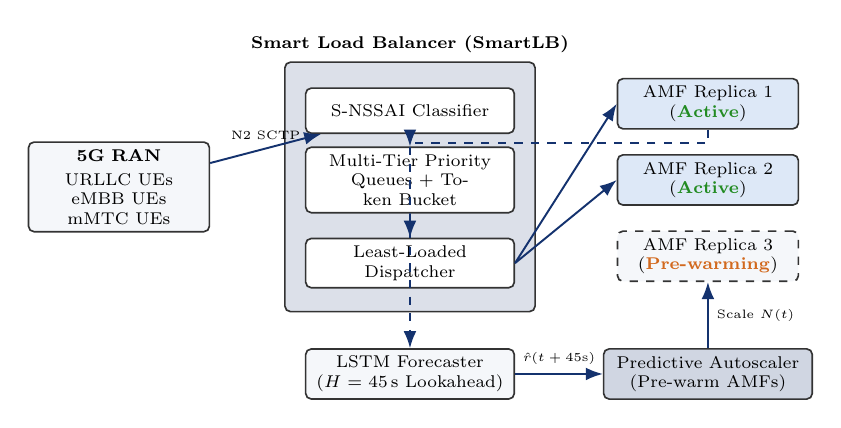
\begin{tikzpicture}[x=1cm, y=1cm, scale=0.88, every node/.style={transform shape}]
    % RAN Layer
    \node[blk, fill=lightgray, text width=2.4cm] (ran) at (-5.0, 0) {\textbf{5G RAN}\\[2pt]URLLC UEs\\eMBB UEs\\mMTC UEs};
    
    % Ingress LB
    \node[blk, fill=primaryblue!15, text width=3.4cm, minimum height=3.6cm] (lb) at (-0.8, 0) {};
    \node[above, font=\scriptsize\bfseries] at (lb.north) {Smart Load Balancer (SmartLB)};
    
    \node[blk, fill=white, text width=2.8cm] (class) at (-0.8, 1.1) {S-NSSAI Classifier};
    \node[blk, fill=white, text width=2.8cm] (pqueue) at (-0.8, 0.1) {Multi-Tier Priority\\Queues + Token Bucket};
    \node[blk, fill=white, text width=2.8cm] (disp) at (-0.8, -1.1) {Least-Loaded Dispatcher};
    
    % AMF Pool
    \node[blk, fill=accentblue!15, text width=2.4cm] (amf1) at (3.5, 1.2) {AMF Replica 1\\(\textcolor{urllcgreen}{\textbf{Active}})};
    \node[blk, fill=accentblue!15, text width=2.4cm] (amf2) at (3.5, 0.1) {AMF Replica 2\\(\textcolor{urllcgreen}{\textbf{Active}})};
    \node[blk, fill=lightgray, text width=2.4cm, dashed] (amf3) at (3.5, -1.0) {AMF Replica 3\\(\textcolor{mmtcorange}{\textbf{Pre-warming}})};
    
    % Scaler & Predictor
    \node[blk, fill=lightgray, text width=2.8cm] (lstm) at (-0.8, -2.7) {LSTM Forecaster\\($H = 45$\,s Lookahead)};
    \node[blk, fill=primaryblue!20, text width=2.8cm] (scaler) at (3.5, -2.7) {Predictive Autoscaler\\(Pre-warm AMFs)};
    
    % Connections
    \draw[flowarr] (ran) -- node[above, font=\tiny] {N2 SCTP} (class);
    \draw[flowarr] (class) -- (pqueue);
    \draw[flowarr] (pqueue) -- (disp);
    \draw[flowarr] (disp.east) -- (amf1.west);
    \draw[flowarr] (disp.east) -- (amf2.west);
    
    \draw[flowarr, dashed] (amf1.south) -- ++(0,-0.2) -| (lstm.north);
    \draw[flowarr] (lstm) -- node[above, font=\tiny] {$\hat{r}(t+45\text{s})$} (scaler);
    \draw[flowarr] (scaler.north) -- node[right, font=\tiny] {Scale $N(t)$} (amf3.south);
  \end{tikzpicture}
\end{frame}

%--------------------------------------------------------------
% Slide 6: Objective 1: S-NSSAI Multi-Tier Queuing
%--------------------------------------------------------------
\begin{frame}{Objective 1: Multi-Tier Slice Queuing}
  \begin{itemize}
    \setlength\itemsep{1.3em}
    \item \textbf{URLLC (Slice 1 -- Mission-Critical):}
      \begin{itemize}
        \item Strict priority zero-queue bypass directly to least-loaded active AMF instance.
        \item 10--15\% capacity headroom permanently reserved across AMF instances.
        \item Strict latency bound guaranteed under 5.0\,ms.
      \end{itemize}
    \item \textbf{eMBB (Slice 0 -- Standard Mobile Broadband):}
      \begin{itemize}
        \item Standard FIFO scheduling queue with round-robin dispatching.
        \item Typical latency target between 10--25\,ms.
      \end{itemize}
    \item \textbf{mMTC (Slice 2 -- Delay-Tolerant IoT):}
      \begin{itemize}
        \item Buffered queue with dynamic token-bucket rate limiting when AMF CPU $> 80\%$.
        \item Starvation protection aging mechanism promotes packets waiting over 5.0\,s.
      \end{itemize}
  \end{itemize}
\end{frame}

%--------------------------------------------------------------
% Slide 7: Objective 1: Scheduling Flowchart
%--------------------------------------------------------------
\begin{frame}{Objective 1: Scheduling Methodology Flow}
  \centering
  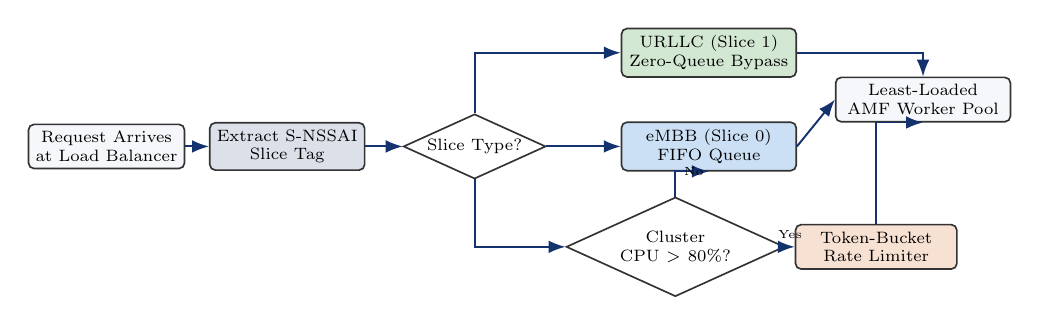
\begin{tikzpicture}[x=1cm, y=1cm, scale=0.85, every node/.style={transform shape}]
    \node[blk] (req) at (0, 0) {Request Arrives\\at Load Balancer};
    \node[blk, fill=primaryblue!15] (parse) at (2.7, 0) {Extract S-NSSAI\\Slice Tag};
    \node[dec] (branch) at (5.5, 0) {Slice Type?};

    \node[blk, fill=urllcgreen!20, text width=2.4cm] (urllc) at (9.0, 1.4) {URLLC (Slice 1)\\Zero-Queue Bypass};
    \node[blk, fill=embbblue!20, text width=2.4cm] (embb) at (9.0, 0.0) {eMBB (Slice 0)\\FIFO Queue};
    \node[dec, text width=2.0cm] (cpu) at (8.5, -1.5) {Cluster\\CPU $> 80\%$?};
    \node[blk, fill=mmtcorange!20, text width=2.2cm] (rate) at (11.5, -1.5) {Token-Bucket\\Rate Limiter};
    \node[blk, fill=lightgray, text width=2.4cm] (pool) at (12.2, 0.7) {Least-Loaded\\AMF Worker Pool};

    \draw[flowarr] (req) -- (parse);
    \draw[flowarr] (parse) -- (branch);
    \draw[flowarr] (branch.north) |- (urllc.west);
    \draw[flowarr] (branch.east) -- (embb.west);
    \draw[flowarr] (branch.south) |- (cpu.west);
    \draw[flowarr] (cpu.east) -- node[above, font=\tiny] {Yes} (rate.west);
    \draw[flowarr] (cpu.north) |- node[right, font=\tiny] {No} (embb.south);
    \draw[flowarr] (urllc.east) -| (pool.north);
    \draw[flowarr] (embb.east) -- (pool.west);
    \draw[flowarr] (rate.north) |- (pool.south);
  \end{tikzpicture}
  \vspace{0.3cm}
  \begin{itemize}
    \item \textbf{URLLC Priority:} Immediate dispatch; bypasses all intermediate queue buffers.
    \item \textbf{mMTC Protection:} Heavy IoT traffic absorbed and regulated without starving standard users.
  \end{itemize}
\end{frame}

%--------------------------------------------------------------
% Slide 8: Objective 2: LSTM Predictive Auto-Scaling
%--------------------------------------------------------------
\begin{frame}{Objective 2: LSTM Predictive Auto-Scaling}
  \begin{itemize}
    \setlength\itemsep{1.2em}
    \item \textbf{Input Observation Window:} Past 60 seconds ($W = 60$\,s) of aggregate arrival rates.
    \item \textbf{Lookahead Prediction Horizon:} Forecasts load $H = 45$\,s ahead ($H \ge T_{\text{boot}} = 40$\,s).
    \item \textbf{Fleet Capacity Dimensioning Formula:}
      \[ N(t) = \left\lceil \frac{\hat{r}(t+H) \cdot (1 + m)}{\mu \cdot \gamma_{\text{target}}} \right\rceil \]
      \begin{itemize}
        \item $\hat{r}(t+H)$: LSTM predicted request rate at future horizon.
        \item $\mu = 100$\,req/s: Maximum service throughput capacity of one AMF instance.
        \item $\gamma_{\text{target}} = 0.80$: Target utilization cap preserving 20\% headroom.
        \item $m = 0.15$: Headroom safety buffer guarding against forecast uncertainty.
      \end{itemize}
    \item \textbf{Hysteresis Stabilization:} 30-second cooldown prevents container flapping.
  \end{itemize}
\end{frame}

%--------------------------------------------------------------
% Slide 9: Scaling Timeline Comparison
%--------------------------------------------------------------
\begin{frame}{Objective 2: Cold-Start Elimination Timeline}
  \centering
  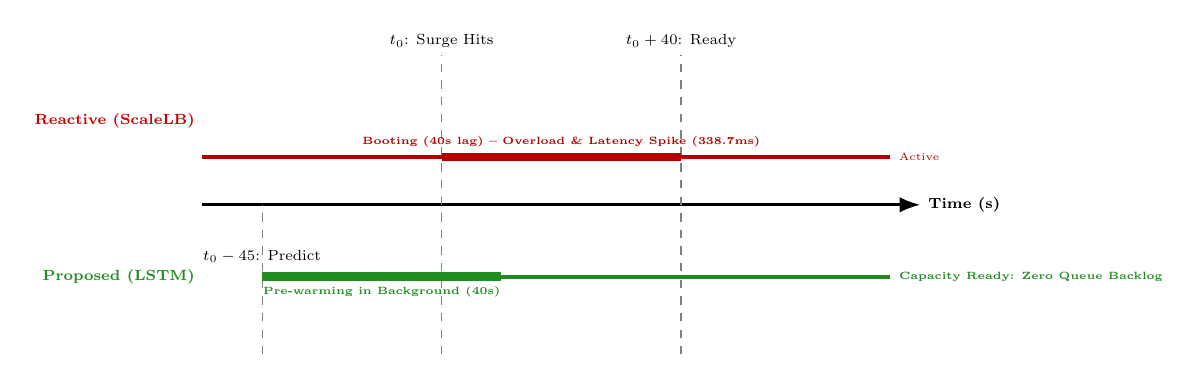
\begin{tikzpicture}[x=1cm, y=1cm, scale=0.76, every node/.style={transform shape}]
    % Time axis
    \draw[-Latex, line width=1pt] (0, 0) -- (12, 0) node[right, font=\scriptsize\bfseries] {Time (s)};
    \draw[dashed, gray] (4, -2.5) -- (4, 2.5) node[above, font=\scriptsize, text=black] {$t_0$: Surge Hits};
    \draw[dashed, gray] (8, -2.5) -- (8, 2.5) node[above, font=\scriptsize, text=black] {$t_0+40$: Ready};

    % Reactive
    \node[left, font=\scriptsize\bfseries, text=red!80!black] at (0, 1.4) {Reactive (ScaleLB)};
    \draw[line width=1.5pt, red!70!black] (0, 0.8) -- (4, 0.8);
    \draw[line width=3pt, red!70!black] (4, 0.8) -- node[above, font=\tiny\bfseries] {Booting (40s lag) -- Overload \& Latency Spike (338.7ms)} (8, 0.8);
    \draw[line width=1.5pt, red!70!black] (8, 0.8) -- (11.5, 0.8) node[right, font=\tiny] {Active};

    % Predictive
    \node[left, font=\scriptsize\bfseries, text=urllcgreen] at (0, -1.2) {Proposed (LSTM)};
    \draw[dashed, gray] (1, -2.5) -- (1, 0) node[below=18pt, font=\scriptsize, text=black] {$t_0-45$: Predict};
    \draw[line width=3pt, urllcgreen] (1, -1.2) -- node[below, font=\tiny\bfseries] {Pre-warming in Background (40s)} (5, -1.2);
    \draw[line width=1.5pt, urllcgreen] (5, -1.2) -- (11.5, -1.2) node[right, font=\tiny\bfseries] {Capacity Ready: Zero Queue Backlog};
  \end{tikzpicture}
  \vspace{0.2cm}
  \begin{itemize}
    \setlength\itemsep{0.4em}
    \item \textbf{Reactive ScaleLB Failure:} Triggers only after surge hits; suffers 54\,s overload and 338.7\,ms tail latency.
    \item \textbf{Predictive Pre-Warming:} New instances boot 45\,s early; full capacity available before traffic arrives.
  \end{itemize}
\end{frame}

%--------------------------------------------------------------
% Slide 10: Implementation & Setup
%--------------------------------------------------------------
\begin{frame}{System Implementation \& Testbed}
  \begin{itemize}
    \setlength\itemsep{0.9em}
    \item \textbf{Docker Microservices Pipeline:}
      \begin{itemize}
        \item \texttt{smart-loadbalancer}: Reverse proxy with S-NSSAI parser, 3 queues, and token bucket.
        \item \texttt{amf-worker}: Scalable container replicas simulating 5G registration procedures.
        \item \texttt{traffic-replayer}: High-throughput workload generator reproducing 3GPP traces.
      \end{itemize}
    \item \textbf{SimPy Discrete-Event Simulation Engine:}
      \begin{itemize}
        \item Replays 240-second flash-crowd surges with deterministic sub-millisecond precision.
        \item Evaluates queuing delay, token replenishments, and 40-second container startup lags.
      \end{itemize}
    \item \textbf{Web Operations Platform:}
      \begin{itemize}
        \item Real-time dashboard with dynamic capacity charts, per-slice KPIs, and container fleet view.
      \end{itemize}
  \end{itemize}
\end{frame}

%--------------------------------------------------------------
% Slide 11: Experimental Results Table
%--------------------------------------------------------------
\begin{frame}{Experimental Results: 320 req/s Surge Benchmark}
  \centering
  \scriptsize
  \begin{tabular}{lccccc}
    \toprule
    \textbf{Configuration} & \textbf{Cold-Start} & \textbf{URLLC p99} & \textbf{mMTC p99} & \textbf{URLLC SLA} & \textbf{AMF-sec} \\
     & \textbf{Lag (s)} & \textbf{Latency} & \textbf{Latency} & \textbf{Compliance} & \textbf{(Cost)} \\
    \midrule
    ScaleLB Reactive (Baseline) & 54\,s & 338.7\,ms & 339.3\,ms & \textcolor{red}{\textbf{FAIL (25.8\% viol.)}} & \textbf{647} \\
    ScaleLB Proactive ($\gamma=0.8$) & 55\,s & 334.1\,ms & 336.5\,ms & \textcolor{red}{\textbf{FAIL (25.8\% viol.)}} & 649 \\
    Warm Standby (1 spare) & \textbf{0\,s} & 32.9\,ms & 32.7\,ms & \textcolor{urllcgreen}{\textbf{PASS (0.0\% viol.)}} & 1024 \\
    O1: Slice Priority Queue Only & 54\,s & 11.1\,ms & 508.6\,ms & \textcolor{urllcgreen}{\textbf{PASS (0.0\% viol.)}} & \textbf{647} \\
    O2: LSTM Prediction Only & 40\,s & 333.1\,ms & 336.5\,ms & \textcolor{red}{\textbf{FAIL (18.3\% viol.)}} & 807 \\
    \textbf{Proposed Full System (O1 + O2)} & \textbf{0\,s} & \textbf{3.15\,ms} & \textbf{499.9\,ms} & \textcolor{urllcgreen}{\textbf{PASS (0.0\% viol.)}} & \textbf{807} \\
    \bottomrule
  \end{tabular}
  \vspace{0.3cm}
  \normalsize
  \begin{itemize}
    \setlength\itemsep{0.4em}
    \item \textbf{Baseline Failure:} ScaleLB suffers 338.7\,ms tail latency and 25.8\% SLA failure.
    \item \textbf{Proposed Success:} Achieves 3.15\,ms URLLC latency with zero cold-start delay.
  \end{itemize}
\end{frame}

%--------------------------------------------------------------
% Slide 12: Key Findings
%--------------------------------------------------------------
\begin{frame}{Key Experimental Takeaways}
  \begin{itemize}
    \setlength\itemsep{1.3em}
    \item \textbf{Complete Cold-Start Elimination:}
      \begin{itemize}
        \item Lookahead prediction ($H = 45$\,s) brings 4 AMF replicas online before surge arrival.
        \item Reduces cold-start overload lag from 54\,s down to \textbf{0\,s}.
      \end{itemize}
    \item \textbf{URLLC 3GPP SLA Compliance:}
      \begin{itemize}
        \item Priority bypass drops 99th-percentile latency from 338.7\,ms to \textbf{3.15\,ms}.
        \item 100\% compliance with 3GPP TS 22.261 sub-5\,ms latency mandate.
      \end{itemize}
    \item \textbf{21.2\% Infrastructure Cost Reduction:}
      \begin{itemize}
        \item Consumes only 807 AMF-seconds compared to 1024 AMF-seconds under Warm Standby.
        \item Avoids wasting CPU and memory on permanently running idle reserve containers.
      \end{itemize}
  \end{itemize}
\end{frame}

%--------------------------------------------------------------
% Slide 13: Operational Dashboard
%--------------------------------------------------------------
\begin{frame}{Operational System Dashboard}
  \begin{columns}[c]
    \column{0.58\textwidth}
    \centering
    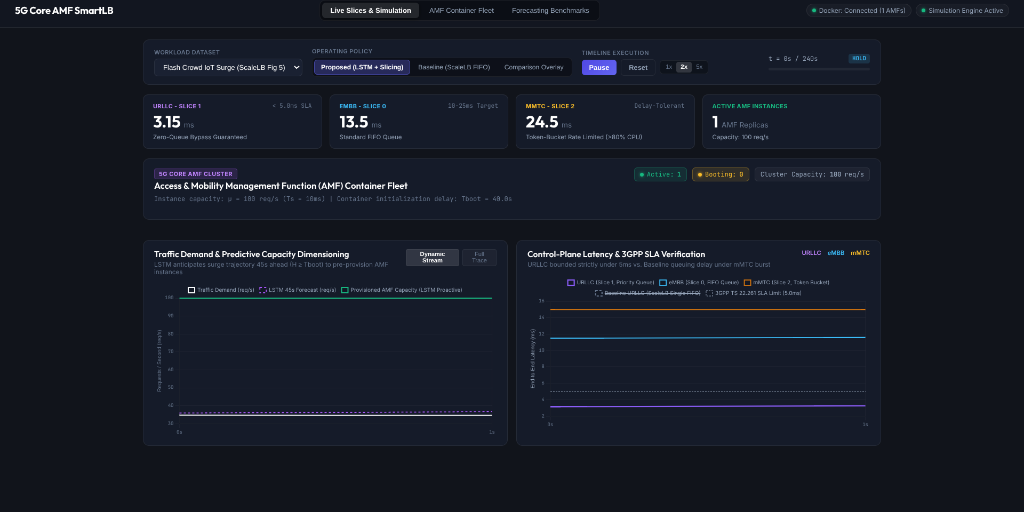
\includegraphics[width=\textwidth]{figures/platform_dashboard.png}
    
    \column{0.42\textwidth}
    \begin{itemize}
      \setlength\itemsep{1.0em}
      \item \textbf{Real-Time Workload Tracking:} Visualizes incoming request rates and 45s predictive trajectory.
      \item \textbf{Fleet Auto-Scaling:} Live display of active, booting, and decommissioned AMF container instances.
      \item \textbf{Latency SLAs by Slice:} Real-time verification of sub-5\,ms URLLC compliance alongside buffered mMTC delay.
    \end{itemize}
  \end{columns}
\end{frame}

%--------------------------------------------------------------
% Slide 14: Conclusion & Future Scope
%--------------------------------------------------------------
\begin{frame}{Conclusion \& Future Scope}
  \begin{itemize}
    \setlength\itemsep{1.3em}
    \item \textbf{Project Summary:}
      \begin{itemize}
        \item Integrated 3GPP S-NSSAI priority queuing with LSTM predictive autoscaling.
        \item Fully eliminated the 40-second container cold-start bottleneck.
        \item Guaranteed 3.15\,ms URLLC latency with zero SLA violations during peak surge.
      \end{itemize}
    \item \textbf{Future Work:}
      \begin{itemize}
        \item \textbf{Multi-Region Federation:} Distribute AMF autoscaling across edge and regional data centers.
        \item \textbf{Kernel-Bypass Ingress:} Implement eBPF/XDP dispatching for line-rate 100\,Gbps processing.
      \end{itemize}
  \end{itemize}
\end{frame}

%--------------------------------------------------------------
% Slide 15: References
%--------------------------------------------------------------
\begin{frame}{References}
  \begin{itemize}
    \setlength\itemsep{1.2em}
    \item \textbf{[1]} W. Dev, S. Bera, and A. Tiwari, \emph{``Control-plane load balancing and auto-scaling in 5G and beyond networks''}, in \emph{Proc. IEEE ICOIN}, 2025, pp. 83--87.
    \item \textbf{[2]} 3GPP, \emph{``Service requirements for the 5G system''}, 3GPP TS 22.261, Release 18, 2023.
    \item \textbf{[3]} Open5GS Project, \emph{``Open source 5G core network implementation''}, \url{https://open5gs.org}.
    \item \textbf{[4]} S. Hochreiter and J. Schmidhuber, \emph{``Long short-term memory''}, \emph{Neural Computation}, vol. 9, no. 8, pp. 1735--1780, 1997.
  \end{itemize}
\end{frame}

\end{document}
